\documentclass{article}

\title{Rendering Translucent Objects using Subsurface Scattering}
\author{Jo\~{a}o Pedro Jorge \and Willem Frishert}
\date{29-01-2007}

\usepackage{subfigure}
\usepackage[pdftex]{graphicx}

\begin{document}
\maketitle

\section{Introduction}
The implemented project goal was to render translucent objects. Those kind of objects can be seen everywhere, and good examples include marble, alabaster, human skin, plants, cloth, jade and many more.
All of the mentioned objects materials have in common the fact that they are not completely opaque due to scattering of light inside of them - know as subsurface scattering. Subsurface scattering causes the diffusion of scattered light and the blurring of small details on the surface of the objects.
Several papers approached these phenomena through the simulation of subsurface scattering. The chosen paper \cite{HierarchicalSSS} was published on SIGGRAPH quite recently and that was the motif that lead to our decision on choosing it. The approach behind the paper extends the diffusion theory present in medical physics related to the measurements of the optical properties of highly scattering materials.


\subsection{BRDF's vs. BSSRDF's}

While the well known BRDF (Bidirectional Reflectance Distribution Function) relates the light incident angle at a certain point with the outgoing angle at that very same point, the BSSRDF (Bidirectional Surface Scattering Reflectance Distribution Function) generalizes that concept and assumes that light might leave the object on a different point on a surface different from the one who arrived at (see Figure \ref{bssrdf_brdf}).

\begin{figure}[hbtp]
  \begin{center}
	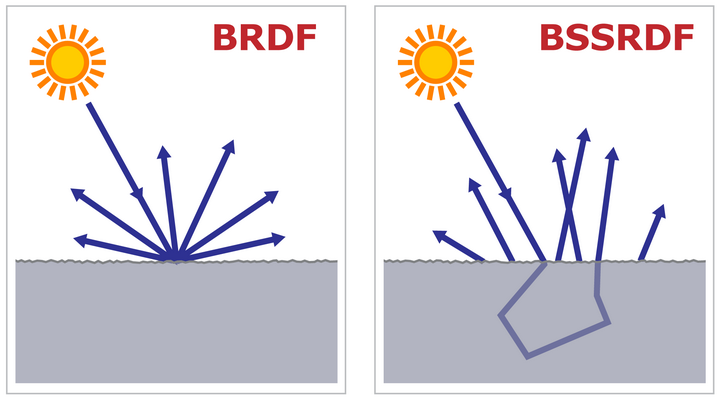
\includegraphics[scale=0.5]{./Pictures/BSSRDF_BRDF.png}
    \caption{BRDF vs BSSRDF Comparison}
    \label{bssrdf_brdf}
  \end{center}
\end{figure}

The BSSRDF, $S$, relates the outgoing radiance, $L _o(x _o, \vec{\omega} _o)$ at the point $x _o$ in the direction $\vec{\omega} _o$, to the incident flux, $\Phi _i(x _i, \vec{\omega} _i)$, at the point $x _i$ from direction $\vec{\omega} _i$:

\begin{equation}
dL _o(x _o, \vec{\omega} _o) = S(x _i, \vec{\omega} _i; x _o, \vec{\omega} _o) d\Phi _i(x _i, \vec{\omega} _i)
\end{equation}

Given a BSSRDF, the outgoing radiance is computed by integrating the incident radiance over incoming directions and area, $A$:

\begin{equation}
L _o(x _o, \vec{\omega} _o) = 
\int_{A}\int _{2\pi} S(x _i, \vec{\omega} _i; x _o, \vec{\omega} _o) L_i(x_i, \vec{\omega_i})(\vec{n} \cdotp \vec{\omega}_i) \,d\omega_i \,dA(x_i)
\end{equation}

\section{Model}
The BSSRDF model used to describe the translucency of a object consists of a sum of two scattering terms: a single scattering term and a diffusion approximation term.\cite{PracticalSSS} The latter term takes into account multiple scattering and is dominant.

\begin{equation}
S(x _i, \vec{\omega} _i; x _o, \vec{\omega} _o) =  {S}_{d}(x _i, \vec{\omega} _i; x _o, \vec{\omega} _o) + {S}^{(1)}(x _i, \vec{\omega} _i; x _o, \vec{\omega} _o)
\end{equation}

Originally, there are 4 parameters that influence the light transport when light hits the object surface and scatters. In \cite{HierarchicalSSS} this is reduced to two parameters: The reduced scattering coefficient ${\sigma}^{\prime}_s$ and the absorption coefficient $\sigma_{ a }$. 


\subsection{The Diffusion Approximation}
The diffusion approximation is based on the observation that light tends to become isotropic when multiple scattering occurs beneath the object surface. To approximate the contribution of the multiple scattering events, a dipole diffusion approximation is used. The dipole comes from medical physics and allows us to compute the radiant exitance for points on the surface.

\subsection{Two-Pass Technique for Evaluating the Diffusion Approximation}
In \cite{PracticalSSS} the diffuse approximation is computed in a single pass  which consumes a fair amount of time. To speed up the computation, Jensen et al. have improved their algorithm in \cite{HierarchicalSSS} by splitting it into a two pass rendering technique. The main idea is to decouple the computation of irradiance from the evaluation of the diffusion approximation. This allows the same irradiance values to be reused for different diffusion approximation evaluations. Besides this, they also improve the efficiency for the evaluation of the diffusion approximation.

\subsubsection{Sampling the Irradiance}
To compute the irradiance on the surface, sample points have to be uniformly distributed over the object surface. The authors propose to use Turk's point repulsion algorithm which uses a relaxation method to spread out the sample points over the surface. The amount of sample points used depends on the surface total area and the mean free path $l_u$. The mean free path stands for the total distance a particle will travel inside the object before is it absorbed. Once the sample points are uniformly spread on the surface we can use global illumination techniques such as photon mapping or irradiance caching to obtain the irradiance at these particular points.
To compute the irradiance on the surface, sample points have to be uniformly distributed over the object surface. The authors propose to use Turk's point repulsion algorithm \cite{Turk_Point_Repulsion} which uses a relaxation method to spread out the sample points over the surface. The amount of sample points used depends on the surface total area and the mean free path $l_u$. The mean free path stands for the total distance a particle will travel inside the object between collisions with other particles. Once the sample points are uniformly spread on the surface we can use global illumination techniques such as photon mapping or irradiance caching to obtain the irradiance at these particular points.

\subsubsection{Evaluating the Diffusion Approximation}
\label{sec:diffaprox}
The Diffusion Approximation can be computed simply by summing the contribution from all the irradiance samples, though that would be computationally expensive, since most objects have thousands of irradiance samples. Using the nearby neighbors could skip some important parts, so an hierarchical evaluation that clusters distant values is the proposed solution in the paper.
For the hierarchical evaluation, an octree is used to store all the irradiance samples. For each voxel, a tuple containing $E_v$, the total irradiance, $A_v$, the total area represented by the points, and $P_v$, the average location weighted by each sample's irradiance value.
In order to evaluate the total radiosity at a location $x$ on the surface of the object, the octree must be traversed starting from the root. For each voxel we test if:

\begin{enumerate}
	\item the location $x$ is inside of it
	\item if not, check if the voxel "is small enough" 
\end{enumerate}

The key idea is that of always subdividing the voxels in the path in which $x$ falls in (until we reach a leaf node). For all the other branches/voxels we need to test the \textit{maximum solid angle $\Delta\omega$} spanned by the points in that particular voxel:

\begin{equation}
\Delta\omega = \frac{A_v}{||x - P_v||^2}
\end{equation}

The value of $\Delta\omega$ must be compared with a certain $\epsilon$ provided by the user. The smaller that $\epsilon$ is, the more accurate and slow the search will be. In Figure \ref{Octree} a typical search can be seen. For the sake of simplicity we have omitted the middle nodes (2 till 7).

\begin{figure}[tbh]
\centering
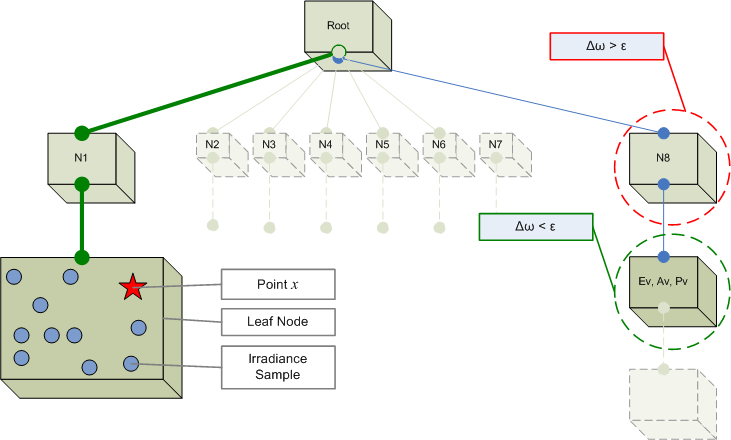
\includegraphics[scale=0.5]{./Pictures/Octree.png}
\caption{Point $x$ (red star) falls on the leftmost node; the other nodes are compared with the $\epsilon$ value until they reach the condition is fulfilled.}
\label{Octree}
\end{figure}

The radiant exitance/radiosity $M_{o,p}$ at $x$ from a given irradiance sample (or for clustered samples, the clustered values) is given by the following equation:

\begin{equation}
M_{o,p}(x) = F_{dt}(x) \frac{dM_o(x)}{d\Phi _i(P_p)\alpha ^{\prime}} E_p A_p
\end{equation}

where $E_p, A_p$ and $P_p$ are the irradiance sample (or clustered sample) values and $\frac{dM_o(x)}{d\Phi _i(P_p)\alpha ^{\prime}}$ can be evaluated using the following equation:

\begin{equation}
\frac{dM_o(x_o)}{d\Phi _i(x_i)\alpha ^{\prime}} = \frac{1}{4\pi}
\left\{ 
z_r ( {\sigma}_{tr} + \frac{1}{d_r} ) \frac{e^{-{\sigma} _{t_r} d_r}}{d _r ^2} + 
z_v ( {\sigma}_{tr} + \frac{1}{d_v} ) \frac{e^{-{\sigma} _{t_r} d_v}}{d _v ^2}
\right\}
\end{equation}

More details about the above parameters can be found in \cite{HierarchicalSSS}.

Finally, the result of traversing and evaluating the voxels is an estimate of the total (diffuse) radiosity, $M_o$ at $x$, which is converted into radiance by:

\begin{equation}
L_o(x,\vec{\omega}) = \frac{F_t(x,\vec{\omega})}{F_{dr}(x)}\frac{M_o(x)}{\pi}
\end{equation}

The parameters that serve passed by the user as an input to these equations are: the  reduced scattering coefficient, ${\sigma} _s ^{\prime}$, the absorption coefficient, ${\sigma} _a$, and the material's index of refraction: $\eta$.

\section{Implementation}
The implementation was initially divided into two parts: uniformly sampling the points and the hierarchical evaluation. However, the point sampling took much more time than it was expected and the work continued in that very same direction. It should be noticed that both of us knew the other one's part and the for several times we worked together in only one part.

The code versioning and backup was done using Google Project Hosting SVN server \cite{SVN}. In this way the synchronization of the code made by both was easy, secure and straightforward.

\subsection{Renderer}
The initial proposal for a renderer mentioned a Pixar's RenderMan{\textregistered} compliant opensource renderer. The choice made was Pixie. The framework seemed to be pretty stable and up-to-date. After several days studying RenderMan{\textregistered}'s specification and trying to understand Pixie's implementation we decided that it was unrealistic to use it due to the lack of documentation and due to Renderman's low support for ray-tracing.

The final choice for a renderer was then PBRT\cite{PBRTBook}. The documentation was excellent and the renderer seemed to be widely used on the academic environment.

Although PBRT is thought to be extended given its plugin nature, modelling a BSSRDF isn't that straightforward (as also mentioned myb the authors on the reference book). Several changes to its core must be made in order to get access to different information. The major changes are related with the {\it Shape, Material, GeometricPrimitive, Triangle and TriangleMesh} objects.

\subsection{First Pass - Sampling The Irradiance}
To obtain the irradiance at specific points on the objects surface, we used Turk's point repulsion algorithm. Firstly, we encapsule the triangles using {\it TriangleUseSets} objects and link them together so the triangles gain more knowledge about their neighbors. A useset also knows information about the triangle such as the normal, the area size and the amount of sample points laying on the triangle surface. Then, in the second part, points are thrown on the triangle mesh and need to be roughly spread. These points are registered in {\it SamplePointContainers} We look a look at some different types of sampling methods and decided in the end to use a low discrepancy sampling method since it was best suited. Then, as Turk's algorithm mentions, we apply a relaxation technique which consist of two parts. Firstly, sample points compute how much force they exert on each other. In order to do this, the triangles, in which the points lay in, have to be transformed to become coplanar. The second part moves the points into the direction force. Either one of thee cases occurs when moving a point: it stays inside the triangle, it moves over the edge of a triangle onto another triangle or it moves over an edge where there is no neighboring triangle. For the last two cases, we used the knowledge provided by the usesets to know what will happen to the point. Either it is moved on the edge of the triangle when there is no neighboring triangle or it is moved over the edge onto the new triangle. Mind that in the latter case, we need to rotate the point around the edge to make sure it falls in the triangle. To debug the position of the sample points we made a small OpenGL application to visualize them. Depending on initial set up of the points on the surface, the relaxation has to be iterated a number of times for the points to settle down. Using the low discrepancy sampling 5 iterators is enough.
In Figure \ref{fig:turk_pointrepulsion_total} the red points are the initial positions where the points start (see Figure \ref{fig:turk_pointrepulsion_before}), the blue points represent the intermediate position of the points during the relaxation iterators (see Figure \ref{fig:turk_pointrepulsion_during}) and the green points are the indicate the final positions(see Figure \ref{fig:turk_pointrepulsion_after}).
\begin{figure}[h]
\centering
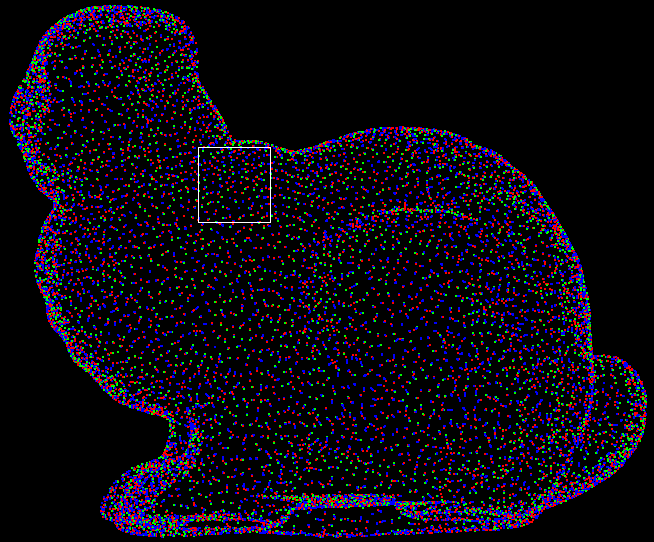
\includegraphics[scale=0.35]{./Pictures/pointrep_total.png}
\caption{Sample points on the bunny after applying point repulsion.}
\label{fig:turk_pointrepulsion_total}
\end{figure}

\begin{figure}[htbp]
  \begin{center}
    \mbox{
      \subfigure[before.] { {\label{fig:turk_pointrepulsion_before}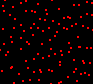
\includegraphics[scale=1.0]{./Pictures/pointrep_before.png}}} \quad 
\subfigure[during.] {\label{fig:turk_pointrepulsion_during} {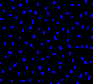
\includegraphics[scale=1.0]{./Pictures/pointrep_during.png}}} \quad
\subfigure[after.] {\label{fig:turk_pointrepulsion_after} {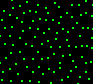
\includegraphics[scale=1.0]{./Pictures/pointrep_after.png}}}
      }
    \caption{Position of sample points per stage.}
    \label{fig:turk_before_during_after}
  \end{center}
\end{figure}

After the sample points have been uniformly spread, the irradiance can be calculated by sampling all the light sources and integrating over the hemisphere:
\begin{equation}
I = \int_{ \Omega  }^{ } L_{sources} \: cos\theta \: sin\theta \:d\phi 
\end{equation}
Monte Carlo estimator can be used to calculate the irradiance by sampling all the radiance from all lights and then dividing this by the amount of samples:
\begin{equation}
I =  \frac{ \pi }{N } \sum_{i=1}^{ N}L_{sources} \left (  \Theta_i  \right )
\end{equation}

\subsection{Second Pass - Evaluating the Diffusion Approximation}
As the authors of the paper, we use an octree to store the irradiance values. Each voxel contains an object, \textit{IrradSample} that stores the 3-tuple spoken on Section  \ref{sec:diffaprox}. For the search another object \textit{IrradProc} is used to retrieve and compute the radiance value for each hit on the object.

The $\epsilon$ value is based on empirical values based on several tests and on the depth of the three used. The latter is computed in order to have a maximum of 8 samples per leaf node:

\begin{equation}
Depth = Round(\log_8(number of samples))
\end{equation}

\section{Results}
The obtained results can be seen on Figures \ref{fig:buddha} and \ref{fig:bunny}. Comparing the obtained results with Jensen's results, we are glad with accomplishments. Some of the results obtained by Jensen can be observed in the original paper \cite{HierarchicalSSS}.

\begin{figure}
\centering
\subfigure[Stanford's Happy Buddha - low resolution picture]{\label{fig:buddha}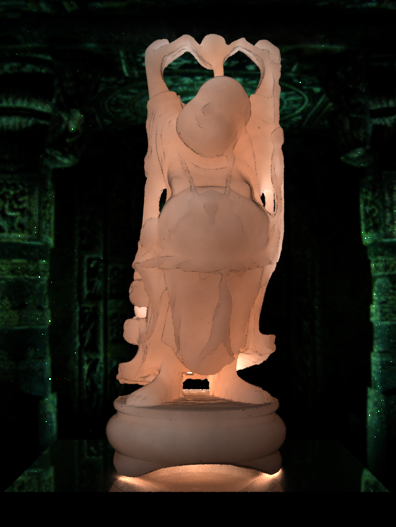
\includegraphics[scale=0.5]{./Pictures/buddha_marble.png}} 
\subfigure[Stanford's Bunny - low resolution picture]{\label{fig:bunny}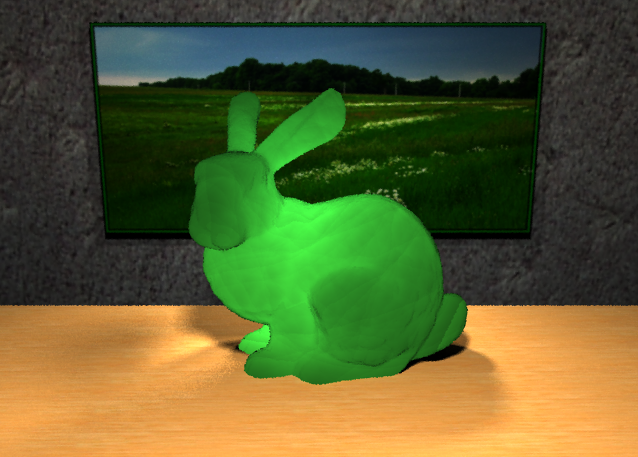
\includegraphics[scale=0.6]{./Pictures/bunny.png}} 
\caption{(a) 300.000 triangles model; rendered in 1 hour. (b) 70.000 triangles (with point repulsion); rendered in 20 minutes.}
\label{fig:ourresults}
\end{figure}

\section{Conclusion}
In this project we have rendered translucent objects with the technique described in \cite{HierarchicalSSS}. The technique has demonstrated to be quite slow, even if some improvements could be made on the code to make it run faster. Furthermore, the results obtained, given the input passed from the user, are quite difficult to predict. The authors provide some measured materials, and given those values we managed to render a Pink Marble Buddha. The rendered picture has some aliasing artifacts due to the fact that the model is not the full resolution version, and therefore some triangles have no area and there are some corrupt normals as well. Much better results would be achieved using the 500.000 triangles model (full resolution Stanford Buddha).

The implemented Turk's Point Repulsion algorithm demonstrated to be quite inefficient for large meshes (more than 100.000 triangles), but we managed to, with only 5 iterations, achieve an excellent result. Unfortunately, this algorithm took half of the development time.

Improvements to our implementation might pass by a more efficient computation of irradiance values and usage of photon mapping to compute those values so we could achieve effects like caustics. Adding specular highlights to the translucent object might as well add some realism in some cases.

% ### BIBLIOGRAPHY ###
\begin{thebibliography}{99}

\bibitem{HierarchicalSSS} Jensen, H.W.  and Buhler, J., 2002, A rapid hierarchical rendering technique for translucent materials. In {\it Proceedings of the 29th annual conference on Computer graphics and interactive techniques SIGGRAPH '02}, ACM Press pp. 576-581.

\bibitem{PracticalSSS} Jensen, H.W., Marschner, S.R., Levoy, M., and Hanrahan, P., 2001, A practical model for subsurface light transport. In {\it Proceedings of the 28th annual conference on Computer graphics and interactive techniques SIGGRAPH '01}, ACM Press pp. 63-69.

\bibitem{SVN} Jorge, J. P., and Frishert, W. 2007. Rendering Translucent Objects SVN Repository. In {\it SVN Repository - http:\slash \slash code.google.com\slash p\slash pbrtbssrdf}.

\bibitem{PBRTBook} Pharr, M., Humphreys, G., 2004, Physically Based Rendering: From Theory To Implementation. The Morgan Kaufmann Series in Interactive 3D Technology.

\bibitem{Turk_Point_Repulsion} Turk G., 1992, Re-tiling polygonal surfaces. In {\it Proceedings of the 19th annual conference on Computer graphics and interactive techniques SIGGRAPH '02}, ACM Press pp. 55-64.

\end{thebibliography}


\end{document}
